%!TEX program=luatex

\newpage
\section{Introduction}
La réalisation d'un logiciel ou d'un système informatique doit être obligatoirement précédée d'une étape d'analyse et de conception qui a pour objectif de définir et de formaliser les étapes nécessaires du développement de l'application afin de rendre cette dernière plus fidèle aux besoins.

La première motivation de ce travail a été de fournir un outil qui permet à l'utilisateur de faire sa revue de presse quotidienne de la façon la plus efficace et la plus enrichissante possible tout en considérant ses centres d'intérêt et préférences. 

Le logiciel que nous proposons enchaîne les processus de catégorisation, de résumé, de traduction et de recommandation d'articles de presse. Pour parvenir à réaliser cet ensemble de tâches en deux langues (Anglais et Arabe), nous allons présenter dans cette partie notre conception qui décrit d'une manière claire et précise le fonctionnement de chaque module du système. 


\section{Module de recommandation}
Dans cette partie, nous allons voir la conception détaillée de notre système de recommandation. Ci-dessous, nous présentons les deux approches proposées, la recommandation personnalisée et non-personnalisée d'articles de presse.
    \subsection{Recommandation personnalisée\label{personal}}
    La recommandation d'articles est basée sur le contenu des profils utilisateurs. En effet, le profilage débute lorsque l'utilisateur s'authentifie pour la première fois et à chaque fois les informations relatives à ses préférences sont récoltées et traitées.

    Cette étape nécessite le profilage des utilisateurs et le calcul de similarité entre ces derniers. Dans ce qui suit les détails de chacune des deux méthodes.

        \subsubsection{Profilage d'un utilisateur}
        Elle consiste à déterminer les centres d'intérêt d'un utilisateur tout en se basant sur les articles lus et visiter. Pour cela, nous avons mis en place plusieurs méthodes de calcul des probabilités de préférences afin de mieux cibler les utilisateurs et garantir une solution conforme aux caractéristiques de la recommandation pour les articles de presse. 

        Pour le calcul des probabilités de préférences utilisateurs, nous avons utilisé une méthode de calcul qui permet à la fois de résoudre le problème de la récence \autoref{recence} et le démarrage à froid \autoref{froid}.

        Le calcul de la probabilité de sélection d'une catégorie pour un utilisateur est basé sur ses interactions avec les articles de presse disponible. Dés qu'un article est sélectionné, l'information est sauvegardée et utilisée pour la mise à jour du vecteur des probabilités de sélection des catégories préférées.

        L'exemple suivant présente un vecteur de probabilité de sélection pour les catégories préférées d'un utilisateur U :
            \[P(U) = {'sport': 0.7178, 'news': 0.1581, 'sci\_tech': 0.1492}\]            
        Il faut noter que la taille du vecteur de probabilité de sélection des catégories préférées est différentes d'un utilisateur à un autre.

        Ce vecteur se met à jour, comme déjà cité, après chaque interaction de l'utilisateur U avec l'article A de la catégorie C. Au fur et à mesure, la probabilité de sélection d'une catégorie C\textsubscript{i} augmente si cette dernière est sélectionnée, sinon, elle diminue pour donner moins d'importances aux articles qui font partie de cette catégorie.

        Ci-après les formules dédiées à la mise à jour des probabilités de sélection des catégories préférées :\\
            \[
            P(U, C) =
            \begin{cases}
                (1-{\alpha}) * {P(U, C)} + {\alpha} & \text{si } \text{article A est sélectionné} \\
                (1-{\alpha}) * {P(U, C)} & \text{sinon.}
            \end{cases}
            \]

        Avec initialement :\\
        \[
        \begin{cases}
            P(U, C) = 1 / \text{NbC } \forall \text{ C} \in \{categorie\textsubscript{1}, categorie\textsubscript{2}, ..., categorie\textsubscript{NbC}\}\\
            NbC : \text{nombre de categories}\\
            \alpha = \text{constante empirique représentant le biais de la diminution}
        \end{cases}
        \]
        \begin{algorithm2e}[H]
        \SetAlgoLined
        \SetKwInOut{Input}{input}
        \SetKwInOut{Output}{output}
        \Input{A: Article, U: Utilisateur}
        \textbf{const :} \alpha = 0.1, NbC = nombre de catégories\\
        préférences = U.préférences\\
        catégorie = A.catégorie\\
        \eIf{catégorie \in préférences}{
            préférences[catégorie] = (1-{\alpha}) * {préférences[catégorie]} + {\alpha}\\
            \While{i < taille(préférences)}{
                \If{préférences[i] != catégorie}{
                    préférences[i] = (1-{\alpha}) * {préférences[catégorie]}\\
                }
            } 
        }
        {
            préférences[catégorie] = 1 / NbC
        }
        \caption{Algorithme de profilage d'un utilisateur}
        \end{algorithm2e}
        \subsubsection{Similarité entre utilisateurs}
        Afin de diversifier la recommandation d'articles de presse, nous avons mis en place une méthode de calcul de similarité entre utilisateur qui permet de recommander des articles selon les préférences et les centres d'intérêt d'un utilisateur similaire. 

        Selon \cite{euclidepreuve} qui propose une étude détaillée sur les mesures de similarité pour le filtrage collaboratif, il en est ressorti comme conclusion que la distance euclidienne était la mesure la plus adéquate en terme de précision et temps d'exécution. La formule de calcul de la distance euclidienne entre les préférences des utilisateurs est la suivante :

        \begin{itemize}[label={}, leftmargin=0cm]
            \item Soient U\textsubscript{1} et U\textsubscript{2} deux utilisateurs,
            \item P(U\textsubscript{1}) et P(U\textsubscript{2}) les vecteurs de probabilité de sélection des catégories préférées des deux utilisateurs respectivement,
            \item NbC\textsubscript{1} et NbC\textsubscript{2} le nombre de catégories préférées de chaque utilisateur,\  
            \item \[Sim({P(U\textsubscript{1})}, {P(U\textsubscript{2})}) = d({P(U\textsubscript{1})}, {P(U\textsubscript{2})}) = {\sqrt {\sum _{i=1, j=1}^{NbC\textsubscript{1},NbC\textsubscript{2}}(P(U\textsubscript{1}, C\textsubscript{i})-P(U\textsubscript{2}, C\textsubscript{j}))^{2}}}\]
        \end{itemize}

        Dans ce qui suit, un exemple de calcul de similarité entre deux utilisateurs :
        \[
        \begin{cases}
            P(U\textsubscript{1}) = {'sport': 0.7581, 'sci\_tech': 0.4492, 'religion': 0.3878, 'algeria': 0.0178,}\\
            P(U\textsubscript{2}) = {'religion': 0.8813,'sport': 0.4421, 'business': 0.3519}\\
        \end{cases}
        \]
        On ignore les probabilités de sélection des catégories non-commune entre les deux utilisateurs.
        \[
        \begin{cases}
        d({'sport'}) = P(U\textsubscript{1},'sport')-P(U\textsubscript{2},'sport') = 0.7581 - 0.4421 = 0.32\\
        d({'religion'}) = P(U\textsubscript{1},'religion')-P(U\textsubscript{2},'religion') = 0.3878 - 0.8813 = −0,49 \\
        Sim({P(U\textsubscript{1})}, {P(U\textsubscript{2})}) = {\sqrt {d({'sport'})^{2}+d({'religion'})^{2}}}= {\sqrt{(0.32)^{2} + (-0.49)^{2}}} = 0,59
        \end{cases}
        \]
        \begin{algorithm2e}[H]
        \SetAlgoLined
        \SetKwInOut{Input}{input}
        \SetKwInOut{Output}{output}
        \Input{A: Article, U: utilisateur}
        \textbf{const :} seuil = 0.1\\
        utilisateurs = Lire(collection de profils)\\
        \While{i < taille(utilisateurs)}{
            \If{utilisateurs[i] != U}{
                sim = distance\_euclidienne(U.préférences, utilisateurs[i].préférences)\\
                \If{sim >= seuil}{
                    U.préférences += utilisateurs[i].préférences
                }
            }
        } 
        \caption{Algorithme de calcul de similarité entre utilisateurs}
        \end{algorithm2e}

    \subsection{Recommandation non-personnalisée}
    La recommandation non-personnalisée vise à recommander des articles pour des utilisateurs qui n'ont pas de comptes (i.e : qui sont non authentifiés), pour cela, notre système effectue une recommandation selon le choix de lecture de l'utilisateur, c'est-à-dire par calcul de similarité entre l'article qui est en train d'être lu et les nouveaux articles disponibles. 

    Un pré-traitement est effectué sur chaque article comprend la suppression des mots vides et l'extraction des racines de mots. Ensuite, le sac à mots (Bag of Words) de l'article est converti en TF-IDF. La matrice résultante de la conversion en TF-IDF est utilisée pour le calcul de la similarité de cosinus et les cinq articles les plus similaires seront recommandés. Le calcul de la similarité entre les articles est présenté ci-dessous.

    \begin{itemize}[label={}, leftmargin=0cm]
        \item Soient U un utilisateur, A\textsubscript{1} et A\textsubscript{2} deux articles de presse,
        \item A\textsubscript{1} a été déjà sélectionné et A\textsubscript{2} est un nouvel article,
        \item BoW(A\textsubscript{1}) et BoW(A\textsubscript{2}) les sacs à mots de chaque article,\\

        \item BoW(A\textsubscript{1}) = \{\begin{arab}'لواء', 'شفيق', 'مدير', 'مكتب', 'رئيس', 'مخلوع', 'مبارك', 'أراد', 'دائم', 'إيقاع', 'عمر', 'سليمان', 'مشير', 'طنطاوي', 'وصف', 'لواء', 'شفيق', 'عاش', 'قصر', 'رئيس', 'مصري', 'مخلوع', 'وفاة', 'عمر', 'سليمان', 'رئيس', 'مخابرة', 'مصري', 'نائب', 'مبارك', 'خسارة', 'أكبر', 'مصر', 'رجل', 'أفضل', 'رجل', 'شجع', 'صعب', 'تعويض', 'تحدث', 'لواء', 'شفيق', 'تصريح', 'علاقة', 'عمر', 'سليمان', 'رئيس', 'مخلوع', 'مبارك'\end{arab}\},

        \item BoW(A\textsubscript{2}) = \{\begin{arab}'استمر' 'نزاع', 'رئيس', 'وزير', 'نوري', 'مالكي', 'شيعي', 'خصم', 'حكم', 'أنصار', 'قائمة', 'عراقي', 'لواء', 'خلفية', 'اتهام', 'مالكي', 'نائب', 'رئيس', 'طارق', 'هاشمي', 'شجع', 'ضلع', 'عملية', 'إرهابي', 'أمر', 'أدى', 'تجميد', 'نشاط', 'حكومة', 'انسحاب', 'وزير', 'قائمة', 'عراقي', 'تفاقم', 'خلاف', 'نظر', 'مطالبة', 'تيار', 'رجل', 'صدري', 'قائمة', 'عراقي', 'علاقة', 'حل', 'برلمان'\end{arab}\},


        \item TF-IDF(A\textsubscript{1}) = \{0.0766346 , 0.05452615 , 0.4598076 , 0.1090523,  0.076346, 0.0766346, 0.0766346, 0.1090523, 0.16357845, ...\},

        \item TF-IDF(A\textsubscript{2}) = \{0.0261347 , 0.156338 , 0.229038 , 0.0730857,  0.0520013, 0.0816399, 0.0261347, 0.2299038, 0.16357845, ...\},

        \item \[sim\_cos(TF-IDF(A\textsubscript{1}), TF-IDF(A\textsubscript{2})) = \frac {TF-IDF(A\textsubscript{1}) \cdot TF-IDF(A\textsubscript{2})}{||TF-IDF(A\textsubscript{1})|| \cdot ||TF-IDF(A\textsubscript{2})||}\]
    \end{itemize}
    \begin{algorithm2e}[H]
        \SetAlgoLined
        \SetKwInOut{Input}{input}
        \SetKwInOut{Output}{output}
        \Input{A: Article, U: utilisateur}
        \Output{ListeArticlesSimilaires: Article}
        articles = Lire(collection d'articles)\\
        \While{i < taille(articles)}{
            segmentation(articles[i])\\
            suppression\_mots\_vides(articles[i])\\
            racinisation(articles[i])\\
        }
        tf-idf = TF-IDF(articles)\\
        mat\_similarité = Tri(cosinus\_similarité(tf-idf))\\
        ListeArticlesSimilaires = mat\_similarité.articles\\
        \Return ListeArticlesSimilaires[:5]
        \caption{Algorithme de calcul de similarité entre articles}
    \end{algorithm2e}

%%~~~~~~~~~~~~~~~~~~~~~~~~~~~~~~~~~~~~~~~~~~~~~~~~~~~~~~~~~~~~~~~~~~~~~~~~~~~~~~~~~~~~~~~~~~~~~~~~~%%
\section{Module de catégorisation d'article de presse}
Le premier module sur lequel nous avons travailler, c'est la catégorisation d'articles de presse. Nous avons expérimenter plusieurs techniques proposées dans la littérature. Nous présentons ci-après chaque approche, ses résultats, ses points forts et ses faiblesses.

    \subsection{Approches expérimentées\label{approches}}
    Toutes les approches utilisées, pour la catégorisation d'articles de presse, sont basées sur l'apprentissage automatique, supervisé et non supervisé. 

    \subsubsection{Basées sur l'Apprentissage Non Supervisé}
        \begin{itemize}
            \item{LDA (Latent Dirichlet Allocation) : }\\
            \textquotedbl Latent Dirichlet Allocation\textquotedbl  est un modèle probabiliste génératif qui permet de décrire des collections de documents de texte ou d'autres types de données discrètes. LDA fait partie d'une catégorie de modèles appelés \textquotedbl topic models\textquotedbl , qui cherchent à découvrir des structures thématiques cachées dans des vastes archives de documents. L'organisation automatique des documents par sujet est une application connue de LDA.
        \end{itemize}
        
    \begin{itemize}[label={}, leftmargin=*]
        \item{\textbf{Corpus et dataset}}\\
        Le Dataset \emph{DeepMind Q\&A} de \cite{cnndailymail} a été utilisé. Les articles de presse ont étaient récoltés pour l'utilisation dans un travail de recherche dans les systèmes de Questions/Réponses. Le corpus est contient 92 579 articles de presse de \emph{CNN}.

        Chaque article est sous le format suivant :
       \begin{itemize}
        \item \textbf{id : }identifiant unique de l'article.
        \item \textbf{contenu : }contenu de l'article.
       \end{itemize}
    \end{itemize}
        
    \subsubsection{Basées sur l'Apprentissage Supervisé}
        \begin{itemize}
            \item{Naïve de Bayes : }\\
            C'est une méthode connue de l'apprentissage automatique supervisé. Un de ses avantages, en plus d'être un modèle simple et facilement interprétable, c'est qu'il renvoie le degré de certitude en plus de la prédiction, ce qui peut être très utile dans certaines applications. 

            Mais en ayant un problème à classes multiples, cette approche nous a donnés des résultats très modeste en un temps d'exécution assez importants, ce qui nous a poussé à abandonner son utilisation.\\
            
            \item{Arbres de décision : }\\
            L'un des algorithmes d'apprentissage automatique supervisé les plus facile à interpréter. Ces principaux avantages sont : robuste face aux données aberrantes, pas très sensible aux données manquantes, possibilité d'intervenir dans la construction de l'arbre, etc. 

            Son principale inconvénient reste la dépendance très forte entre la taille de la base d'apprentissage et les performances.\\
            
            \item{SVM (Support Vector Machines) : }\\
            Les machines à vecteurs supports (en anglais Support Vector Machine, SVM) sont destinées à résoudre des problèmes de classification et de régression. Les SVMs cherchent à trouver la frontière séparatrice optimale entre les classes, à partir d'un ensemble d'apprentissages. Dans le cas de la classification de textes (articles de presse dans notre cas), les SVMs ont montrés une grande capacité de prédiction malgré le très grand nombre de caractéristiques des textes (> 10000) contrairement aux autres techniques.\\ 
            
            \item{Descente de Gradient Stochastique : }\\
            Le SGD est un algorithme de classification linéaire, souvent utilisé pour l'optimisation. Il peut être combiné avec d'autres techniques d'apprentissage, (SVM, Réseau de neurones, etc.), comme  fonction d'optimisation d'erreur. Dans notre cas, il est utilisé avec un SVM pour le modèle de catégorisation d'articles de presse arabe.
        \end{itemize}

    \begin{itemize}[leftmargin=*, label={}]
        \item{\textbf{Corpus et dataset}}\\
            Nous avons défini une structure pour chaque article, pour faciliter l'exploration des datasets. Ci-dessous la structure choisie :
            \begin{itemize}
               \item{\textbf{id} : }un identifiant unique de l'article,
               \item{\textbf{contenu} : }les différents paragraphes de l'article,
               \item{\textbf{catégorie} : }la catégorie de l'article extraite depuis la source.
            \end{itemize}
    \end{itemize}

    \subsection{Processus de catégorisation}
        \subsubsection{Pré-traitement des articles de presse}\label{pretraitement}
        Plusieurs opérations de pré-traitements ont été effectuées sur chaque article dans le but de rendre l'utilisation des données avec les différents algorithmes d'apprentissage automatique possible.

        On prend le paragraphe suivant comme exemple :

            \begin{arab}أمرت السلطات القطرية الأسواق والمراكز التجارية في البلاد برفع وإزالة السلع الواردة من السعودية والبحرين والإمارات ومصر في الذكرى الأولى لإعلان هذه الدول الحصار عليها.\end{arab}
            
        Ci-après les étapes de pré-traitement suivies :
        \begin{enumerate}[leftmargin=*]
            \item{\textbf{Segmentation (Tokenization) et suppression des mots vides :} }permet d'extraire toutes les entités lexicales d'un article donné. La segmentation est suivie de la suppression des tokens non-utiles tel que la ponctuation, les pronoms, les déterminants, etc.

            Après segmentation : 
                \begin{arab}'أمرت', 'السلطات', 'القطرية', 'الأسواق', 'و', 'المراكز', 'التجارية', 'في', 'البلاد', 'برفع', 'و', 'إزالة', 'السلع', 'الواردة', 'من', 'السعودية', 'و', 'البحرين', 'و', 'الإمارات', 'و', 'مصر', 'في', 'الذكرى', 'الأولى', 'لإعلان', 'هذه', 'الدول', 'الحصار', 'عليها', '.'\end{arab}
            

            Après suppression des mots vides : 
            \begin{arab}'أمرت', 'السلطات', 'القطرية', 'الأسواق', 'المراكز', 'التجارية', 'البلاد', 'برفع', 'إزالة', 'السلع', 'الواردة', 'السعودية', 'البحرين', 'الإمارات', 'مصر', 'الذكرى', 'الأولى', 'لإعلان', 'الدول', 'الحصار'\end{arab}
            
            
            \item{\textbf{Racinisation (Stemming) :} }les mots d'un document sont représentés par leurs racines plutôt que par les mots d'origine. Plusieurs variantes d'un terme peuvent ainsi être groupées dans une seule forme représentative, ce qui réduit le nombre des termes distincts nécessaires pour représenter un document.

            Après racinisation : 
            \begin{arab}'أمر', ' سلطة ', 'قطر', 'سوق', 'مركز', 'تجاري', 'بلد', 'رفع', 'إزالة', 'سلعة', 'وارد', 'سعودية', 'بحرين', 'إمارة', 'مصر', 'ذكرى', 'أول', 'إعلان', 'دولة', 'حصار'\end{arab}
            

            \item{\textbf{N-grammes :} }les N-grammes permettent de construire une sous-séquence de n mots consécutifs. Ils permettent de contextualiser l'ordre d'apparition d'un ensemble de mots.

            Après génération des N-grammes (bi-grammes dans notre cas) : 
            \begin{arab}('أمر', 'سلطة'), ('سلطة', 'قطر'), ('قطر', 'سوق'), ('سوق', 'مركز'), ('مركز', 'تجاري'), ('تجاري', 'بلد'), ('بلد', 'رفع'), ('رفع', 'إزالة'),('إزالة', 'سلعة'), ('سلعة', 'وارد'), ('وارد', 'سعودية'), ('سعودية', 'بحرين'), ('بحرين', 'إمارة'), ('إمارة', 'مصر'), ('مصر', 'ذكرى'), ('ذكرى', 'أول'), ('أول', 'إعلان'), ('إعلان', 'دولة'), ('دولة', 'حصار')\end{arab}
            
        \end{enumerate}
        \subsubsection{Modèle de classification d'articles de presse}
            Nous avons développé plusieurs modèles de catégorisation d'articles de presse basés sur l'apprentissage supervisé et non supervisé présentés dans la \autoref{approches}. L'algorithme \autoref{algomodeles} présente les étapes de développement des différents modèles.

            \begin{algorithm2e}[H]
            \label{algomodeles}
            \SetAlgoLined
            \SetKwInOut{Input}{input}
            \SetKwInOut{Output}{output}
            \Input{Dataset: Article}
            \Output{ModèleEntrainé}
            tf-idf = [ ]\\
            \For{article \in Dataset}{
                segmentation(article)\\
                suppression\_mots\_vides(article)\\
                racinisation(article)\\
                n-grammes(article)\\
                tf-idf += TF-IDF(article)
            }
            ModèleEntrainé = AlgorithmeClassification(tf-idf)\\
            \Return{ModèleEntrainé}
            \caption{Algorithme de construction des modèles de catégorisation}
            \end{algorithm2e}

        \subsubsection{Prédiction des catégories d'articles de presse}
            Une fois le modèle est prêt, nous utilisons le résultat pour la prédiction d'un nouvel article. L'article à classifier doit passé par les mêmes étapes de pré-traitement cités dans la \autoref{pretraitement}. On peut voir le processus de la prédiction dans l'algorithme \autoref{algoprediction}.

            \begin{algorithm2e}[H]
            \label{algoprediction}
            \SetAlgoLined
            \SetKwInOut{Input}{input}
            \SetKwInOut{Output}{output}
            \Input{A: Article}
            \Output{catégorie: Catégorie}
            segmentation(A)\\
            suppression\_mots\_vides(A)\\
            racinisation(A)\\
            n-grammes(A)\\
            prédiction = Charger(modèle)\\
            catégorie = prédiction(A)\\
            \Return{catégorie}
            \caption{Algorithme de prédiction de catégorie d'un article de presse}
            \end{algorithm2e}
%%~~~~~~~~~~~~~~~~~~~~~~~~~~~~~~~~~~~~~~~~~~~~~~~~~~~~~~~~~~~~~~~~~~~~~~~~~~~~~~~~~~~~~~~~~~~~~~~~~%%

\section{Module de résumé automatique}
Le résumé automatique permet à l'utilisateur de notre système d'avoir une idée générale sur le contenu d'un article de presse. Les idées les plus importantes d'un texte sont identifiées. Afin de réussir l'identification des idées (phrases ou mots), nous avons expérimenté plusieurs techniques que nous allons présenter dans ce qui suit.

    \subsection{Résumé extractif par Apprentissage Supervisé}
    Tout d'abord, nous avons commencé par l'approche proposée dans \cite{riad-belkbir} qui est basée sur un apprentissage automatique supervisé en utilisant un dataset annoté manuellement. 
        \subsubsection{Corpus et datasets}
        Le dataset développé par l'équipe TALAA, contient plus de 70 articles. Il est dédié principalement au résumé automatique par apprentissage supervisé pour la langue Arabe, mais peut être utilisé également dans d'autres applications, telles que la compression des textes.

        L'annotation consiste en l'attribution de quatre types d'étiquettes possibles à chaque phrase de l'article :
            \begin{itemize}
                \item S (select) : phrase importante, à prendre en considération dans la construction du résumé.
                \item R (remove) : cette phrase est à supprimer, son absence n'affecte pas le sens du résumé.
                \item F (fusion) : fusion de deux phrases (ou plus).
                \item C (compress) : compression d'une phrase, on supprimant les synonymes et les redondances dans le sens.\\
            \end{itemize}

        \subsubsection{Pré-traitement et structure du dataset}
        Tout les articles du dataset sont sous le format XML, chaque article a son propre identifiant et divisé en paquets de phrases selon l'opération effectuée. Ci-après la \autoref{xml-structure} qui montre un exemple du dataset : 
        \begin{figure}[H]
            \centering
            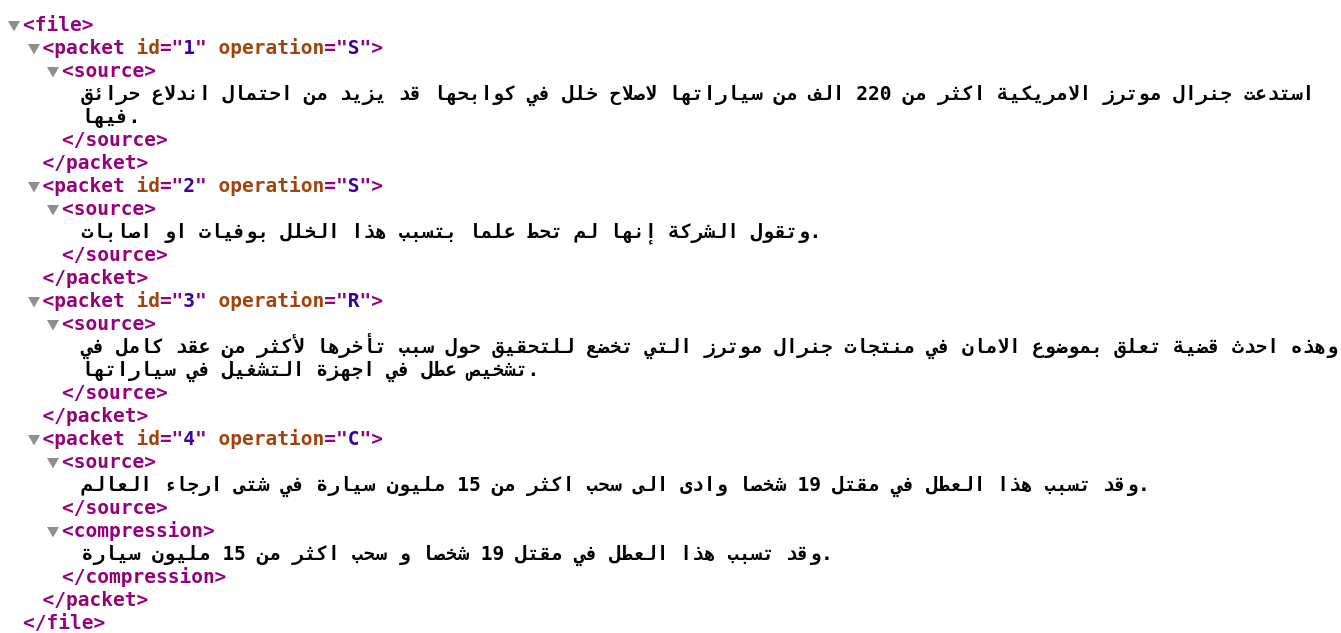
\includegraphics[height=220pt,width=430pt]{img/chapter4/xml.png}
            \caption{Structure d'un article du dataset de résumé automatique}
            \label{xml-structure}
        \end{figure}
        L'approche basée sur l'apprentissage automatique demandait un très grand nombre d'articles avec leurs résumés, ce qui nous a poussés à l'abandonner.

    \subsection{Résumé extractif par Machine de Boltzman}
    L'approche proposée dans \cite{boltzman} utilise un modèle d'apprentissage profond afin de prédire les phrases les plus importantes dans un texte donnée en utilisant 9 caractéristiques sur chaque phrase. Elle consiste en trois grandes phases: l'extraction des caractéristiques, la conversion en valeurs numériques et la génération du résumé à partir des scores de chaque phrase. 

    Les caractéristiques extraites sont les suivantes :
    \begin{enumerate}
        \item{Nombre de mots clés}
        \item{Position de la phrase dans le texte}
        \item{Longueur de la phrase}
        \item{Position de la phrase dans le paragraphe}
        \item{Nombre de noms propres}
        \item{Nombre d'entités numériques}
        \item{Nombre d'entités nommées}
        \item{TF-ISF (Term Frequency- Inverse Sentence Frequency)}
        \item{Similarité avec la phrase centroïde}
    \end{enumerate} 

    \subsection{Résumé automatique extractif par plongement de mots}
    L'approche proposée par l'équipe de recherche du département informatique de l'Université de Bari en Italie \cite{notreresume}, est basée sur la similarité textuelle entre la phrase centroïde et les autres phrases du texte en utilisant les plongements de mots (Word embeddings) présentés dans \autoref{wordebd}. Le plongement de mots utilisé dans cette approche est un modèle Skip-Gram (\autoref{skip-gram}) entraîné sur le contenu de Wikipédia en utilisant la bibliothèque FastText développé par le Laboratoire en Intelligence Artificielle de \emph{Facebook} qui prend en charge 294 langues différentes \cite{fasttext}. Parmi les modèles développés, nous allons nous intéresser à celui de l'Anglais et l'Arabe. Ci-dessous, nous allons présenter les étapes de conception du résumé automatique.

        \subsubsection{pré-traitement des articles}
        Dans cette phase, il suffit juste de segmenter les textes en phrases, les phrases en tokens et supprimer les mots vides. Ceci étant dû au fait que le plongement de mots que nous allons utiliser (le modèle Skip-Gram entraîné sur le contenu Wikipédia) servira entre autres à détecter les régularités linguistiques des  mots de la même racine. Par exemple : le mot le plus similaire à \textquotedbl Algeria\textquotedbl est le mot \textquotedbl Algerian\textquotedbl \ref{}, c'est pour cela que la racinisation n'est pas utilisée. L'algorithme \autoref{algopreresume} décrit les étapes de pré-traitement d'un article.

         \begin{algorithm2e}[H]
          \label{algopreresume}
          \SetAlgoLined
          \SetKwInOut{Input}{input}
          \SetKwInOut{Output}{output}
          \Input{A: Article}
          \Output{ListeTokens: token}
          Lire(A)\\
          phrases = segmentation(A)\\
          \For{phrase \in phrases}{
            tokens = tokenisation(phrase)\\
            ListesTokens += suppression\_mots\_vides(tokens)\\
          }
          \Return {ListesTokens}
         \caption{Algorithme de pré-traitement du résumé}
        \end{algorithm2e}

       \subsubsection{Construction d'un vecteur de centroïde}
        Après l'étape de pré-traitement, place à la construction des vecteurs de centroïde. Afin de construire un vecteur centroïde en utilisant les plongements de mots, nous sélectionnons d'abord les mots significatifs dans le document. Pour cela, nous calculons le poids TF-IDF de chaque mot dans chaque document. Ensuite, les mots ayant le poids TF-IDF supérieur à une constante empirique fixée au tout début de cette phase qui désignera un seuil de document (IDF) seront sélectionnés. Ainsi, nous calculons l'encastrement du centroïde comme la somme des mots les mieux classés dans le document en utilisant les plongements de mots de Wikipédia, comme le montre l'équation suivante :

             \begin{equation*}
             C = \sum_{\substack{w\in D\\
                             tf-idf(w)>t }}
                    E[idx(w)]
             \end{equation*}
             
             Où :
             C: l'encastrement centroïde lié au document D.\\
             idx(w) : une fonction qui retourne l'indice du mot dans le vocabulaire.\\
             
             \begin{algorithm2e}[H]
                \SetAlgoLined
                \SetKwInOut{Input}{input}
                \SetKwInOut{Output}{output}
                \Input{phrases, SeuilDocument}
                \Output{Vecteur centroïde}
                
                Lire(phrases)\\
                \For{phrase \in phrases}{
                    \For{mot \in phrase}{   
                    tf-idf=CalculTfIdf(mot)\\
                    \If{tf-idf > seuilDocument}
                    {
                    Séléction += mot
                    }
                 }
             }
                
                Encastrement=SommeVecteurs(Séléction)
                
                \Return{Encastrement}
                \caption{Algorithme de construction du vecteur centroïde}
             \end{algorithm2e}
             
             \vspace*{0.5cm}
             La \autoref{centro-vec} présente un exemple d'un vecteur de centroïdes. 
              \begin{figure}[H]
                 \centering
                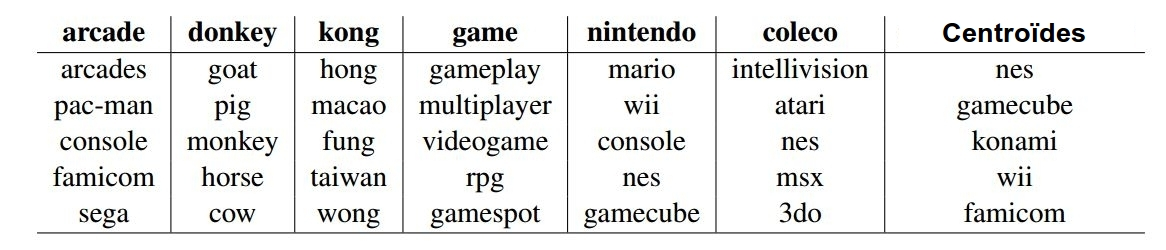
\includegraphics[height=95pt,width=420pt]{img/chapter3/centroideembed.jpg}
                \caption{Vecteurs de centroïdes - Table 1, page 14 \ref{plongement}}
                \label{centro-vec}
             \end{figure}
         \vspace*{1cm}    
         \subsubsection{Notation des phrases}
         Après l'étape de construction du vecteur centroïde, la somme des plongements de mots de chaque terme  est attribuée à la phrase où il apparaît.\label{somplong}

        \begin{equation*}
         S\textsubscript{j} = \sum_{\substack{w\in S\textsubscript{j}}}
         E[idx(w)]
        \end{equation*}
        Où :
        S\textsubscript{j}: la $j\textsuperscript{ième}$ phrase du document. \\ 
        $E[idx(w)]$ : le plongement de mot du terme $w$.

        Afin d'obtenir le score finale de la phrase, on calcule la similarité de cosinus entre la somme des plongements, déjà calculé (\ref{somplong}), de la phrase S\textsubscript{j} et le plongement de la phrase centroïde S\textsubscript{centroide}.
        
        \[sim\_cos(S\textsubscript{centroide},S\textsubscript{j}) = \frac {S\textsubscript{centroide} \cdot S\textsubscript{j}}{||S\textsubscript{centroide}|| \cdot ||S\textsubscript{j}||}\]

        La \autoref{notation-phrase} présente un exemple de plongement de mots.
            \begin{figure}[H]
                \centering
                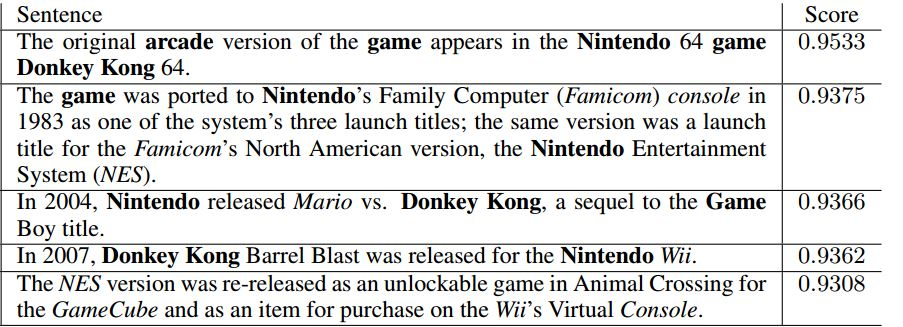
\includegraphics[height=155pt,width=400pt]{img/chapter3/scoreembed.jpg}
                \caption{Notation des phrases - Table 2, page 14 \ref{plongement}}
                \label{notation-phrase}
            \end{figure}

        \subsubsection{Sélection des phrases}
       Après la phase de notation des phrases du document, elles sont, ensuite, triées par ordre décroissant en fonction de la similarité. Les phrases les mieux classées sont itérativement sélectionnées et ajoutées au résumé jusqu'à ce que la limite (taille du résumé) soit atteinte. Afin de satisfaire la propriété de redondance, nous allons calculer, à chaque itération, la \emph{similarité de cosinus} entre la phrase à venir et les phrases déjà sélectionnées dans le résumé.\\
       Il est à noter qu'un seuil a été fixé afin de rejeter toutes les phrases qui ont une similarité très élevées par rapport à une phrase afin d'éviter cette redondance.
        \begin{algorithm2e}[H]
            \SetAlgoLined
            \SetKwInOut{Input}{input}
            \SetKwInOut{Output}{output}
            \Input{phrases, scores, seuilSimilarité, seuilRésumé}
            \Output{Résumé}
            phrases = Tri(phrases, scores)\\
            k = 1\\
             \For{i=1 \KwTo taille(phrases)}{                
                \If{taille(Résumé) > seuilRésumé}{
                    \Return Résumé\\
                    sv = sommeVecteurs(phrases[i])\\
                    prendrePhrase = Vrai\\
                }
                \For{j=1 \KwTo k}{
                    sv2 = sommeVecteurs(Résumé[j])\\
                    sim = similarité(sv, sv2)\\
                    \If{sim > seuilSimilarité}{
                        prendrePhrase = Faux\\
                    }
                }
                \If{prendrePhrase}{
                    Résumé[k] = phrases[i]\\
                    k += 1\\      
                }
             }
             \Return{Résumé}
            \caption{Algorithme de Sélection des phrases}
        \end{algorithm2e}

        À la fin de cette étape, nous allons avoir un résumé du document désordonné et les phrases sont triées selon leur score et pas dans l'ordre de leurs apparitions dan le texte original. Pour y remédier, nous allons rajouter un tri des phrases selon l'ordre du document.
        
         \begin{algorithm2e}[H]
             \SetAlgoLined
             \SetKwInOut{Input}{input}
             \SetKwInOut{Output}{output}
             \Input{Résumé}
             \Output{RésuméTrié}
             RésuméTrié = Tri(Résumé, ordreApparitionPhrases)\\
              \Return{RésuméTrié}
             \caption{Algorithme de génération du résumé automatique}
         \end{algorithm2e}

\section{Module de traduction}
Dans ce module, notre tâche n'était pas d'implémenter ou de concevoir un traducteur automatique, mais uniquement d'utiliser un traducteur multilingue existant, et de l'intégrer dans notre architecture globale présentée dans la \autoref{shemaglobal}. 
Toutefois, il fallait rechercher le module de traduction le plus performant afin de traduire un article complet de la manière la plus rapide.

Afin d'intégrer un bon système de traduction automatique, nous avons exploré deux sources principales, la première était destiné à une utilisation professionnelle, de plus, la version gratuite offrait une traduction pour des textes de taille limités. Et la deuxième, était la solution la plus adaptée à notre cas d'étude. Elle est à la fois accessible et offrait des possibilités de traduction pour des textes longs (articles de presse, thèse, etc). 

\section{Conception de la base de données}
Afin de s'adapter à la structure très dynamique des articles de presse et des profils également, nous avons choisi d'utiliser les bases de données NoSQL\ref{nosql}.

Le SGBD MongoDB que nous avons utiliser est un système orienté document écrit en C++ \cite{NOSQL3}. Les objets sont stockés en série sous la forme BSON\footnote{C'est un format d'échange de données informatiques utilisé principalement comme stockage de données et format de transfert de données par le réseau dans la base de données MongoDB [Wikipédia]}

Les objets n'ont pas besoin d'avoir la même structure ou les mêmes champs et les champs communs n'ont pas besoin d'avoir le même type, permettant ainsi un stockage de schéma flexible. À cet effet, nous présentons ci-dessous, sous notre base de données, la collection d'articles et la collection des profils.

\subsection{Collection d'articles}
Les articles extraits depuis différentes sources sont tous sauvegardés sous une structure définie au préalable, prenant en considération les différences entre les formats suivies par les revues de presse. 

À cet effet, nous avons choisi \emph{JSON} qui est un format léger d'échange de données. Il est facile à lire ou à écrire pour des humains \cite{json} et est pris en charge par tout les langages de programmation.

Chaque article est représenté comme suit :
\begin{itemize}
    \item \textbf{Identifiant, \textquotedbl \_id\textquotedbl: } identifiant unique d'un article de presse.
    \item \textbf{Langue, \textquotedbl language\textquotedbl:} la langue dans laquelle l'article est écrit.
    \item \textbf{Titre, \textquotedbl title\textquotedbl:} le titre de l'article.
    \item \textbf{Source, \textquotedbl source\textquotedbl:} nom de la revue de presse source.
    \item \textbf{Auteur, \textquotedbl author\textquotedbl:} on sauvegarde le nom de l'auteur.
    \item \textbf{Contenu, \textquotedbl content\textquotedbl:} contenu de l'article de presse.
    \item \textbf{Horaire, \textquotedbl publishedAt\textquotedbl:} date et heur local de publication.
    \item \textbf{Lien de l'article, \textquotedbl url\textquotedbl:} lien vers la page de l'article originale.
    \item \textbf{Lien de l'image, \textquotedbl urlToImage\textquotedbl:} lien vers l'image principale de l'article originale.
    \item \textbf{Catégorie, \textquotedbl categoryPredicted\textquotedbl:} catégorie de l'article inférée en utilisant nos modèles.
    \item \textbf{Résumé, \textquotedbl summaryGenerated\textquotedbl:} résumé automatique générée.
    \item \textbf{Traduction, \textquotedbl translatedContent\textquotedbl:} contenu de l'article de presse traduit.\\
\end{itemize}

Voici maintenant un exemple d'un document de la collection d'articles :
\begin{lstlisting}[style=code]
{
'_id': '5afc18571d41c833a8632a24', 
'language': 'en',
'title': "Smart's stellar Game 2 play draws Cavs praise", 
'source': 'espn', 
'author': 'Chris Forsberg', 
'content': 'LeBron James and Tyronn Lue explain what they think of Marcus...'
'publishedAt': '2018-05-16T05:48:55Z', 
'url': 'http://espn.go.com/nba/id/235168',
'urlToImage': 'http://espn.go.com/nba/id/235168/main.png',  
'categoryPredicted': 'sport', 
'summaryGenerated': 'The Celtics improved to 8-2 since Smart returned...', 
'translatedContent': 'Les Celtics ont enchainé, depuis le retour de Smart...', 
},
\end{lstlisting}

\subsection{Collection de profils}
Le profil d'utilisateur regroupe très peu d'informations dans le but de protéger la vie privée. Cependant, les catégories et les sources préférées par l'utilisateur sont sauvegardées. 

Un profil utilisateur est représenté comme suit :
\begin{itemize}
    \item \textbf{Identifiant, \textquotedbl  \_id\textquotedbl : } identifiant unique.
    \item \textbf{Nom d'utilisateur, \textquotedbl  username\textquotedbl : } nom d'utilisateur unique.
    \item \textbf{Mot de passe, \textquotedbl  password\textquotedbl : } mot de passe pour l'authentification crypté.
    \item \textbf{Adreese mail, \textquotedbl  email\textquotedbl : } email de l'utilisateur.
    \item \textbf{Catégories préférées, \textquotedbl  preferences\textquotedbl : } vecteurs de catégories préférées .
    \item \textbf{Sources préférées, \textquotedbl  sources\textquotedbl : } noms des sources de revues de presse préférées. 
\end{itemize}

Ci-dessous un exemple d'un document de la collection de profils :
\begin{lstlisting}[style=code]
{
'_id': '5afc18571d41c833a8632a24', 
'username': 'yankheloufi'
'password': 'CAESEMgZsfgjSKT7GvZNAtFJaAs'
'email': 'yk@usthb.dz',
'preferences': {'entertainment': '0.63','world': '0.42','health': '0.12'},
'sources': ['wello-mag', 'al-jazeera-english', 'bbc-news'],
},
\end{lstlisting}


\section{Architecture du système \textquotedbl Feedny\textquotedbl}
Dans cette partie, nous allons présenter l'architecture globale de notre système, cette dernière est déployée sous la forme d'une architecture 3-tiers. Ci-dessous, nous présentons ce qu'est une architecture 3-tiers ainsi que son avantage avant d'expliciter un schéma de l'architecture globale.

\subsection{Présentation de l'architecture 3-tiers}
Une application mobile ou web possède souvent une architecture 3-tiers.
\begin{itemize}
    \item\textbf{La couche DAO : }\\
    \textquotedbl Data Access Object\textquotedbl  s'occupe de l'accès aux données, le plus souvent des données persistantes au sein d'un SGBD.\\
    \item\textbf{La couche métier : }\\
    Implémente les algorithmes \textquotedbl métiers\textquotedbl  de l'application. Cette couche est indépendante de toute forme d'interface avec l'utilisateur. C'est généralement la couche la plus stable de l'architecture. Elle ne change pas si on change l'interface utilisateur ou la façon d'accéder aux données nécessaires au fonctionnement de l'application.\\
    \item\textbf{La couche interface utilisateur : }interface (web ou mobile) qui permet à l'utilisateur de piloter l'application et d'en recevoir des informations.
\end{itemize}

\begin{figure}[H]
    \centering
    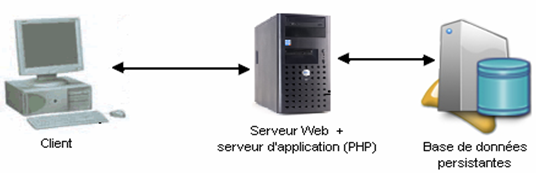
\includegraphics[height=100pt,width=400pt]{img/chapter3/tiers.png}
    \caption{Architecture 3-tiers}
\end{figure}

\subsection{Avantage de l'architecture multi-tiers}
L'avantage principal d'une architecture 3-tiers (multi-tiers) est la facilité de déploiement. L'application
en elle même n'est déployée que sur la partie serveur. Le client ne nécessite qu'une installation et une configuration minime. 

Cette facilité de déploiement aura pour conséquence non seulement de réduire le coût de déploiement, mais aussi de permettre une évolution régulière du système. Cette évolution ne nécessitera que la mise à jour de l'application sur le serveur applicatif.

\subsection{Schéma global de \textquotedbl Feedny\textquotedbl}
L'architecture globale du système \textquotedbl Feedny\textquotedbl  comporte quatre processus principaux: catégorisation, résumé, traduction et recommandation d'articles de presse.

Les entrées (articles de presse extraits de plusieurs sources) sont sauvegardées dans une base de données. Le processus de catégorisation commence par classifier l'article selon son contenu, ensuite un résumé est généré, l'article est traduit de l'Anglais vers l'Arabe (ou l'inverse) et enfin, il sera recommandé à un utilisateur selon son profil et ses préférences comme on peut le voir dans la figure \ref{shemaglobal}.

\begin{figure}[H]
    \centering
    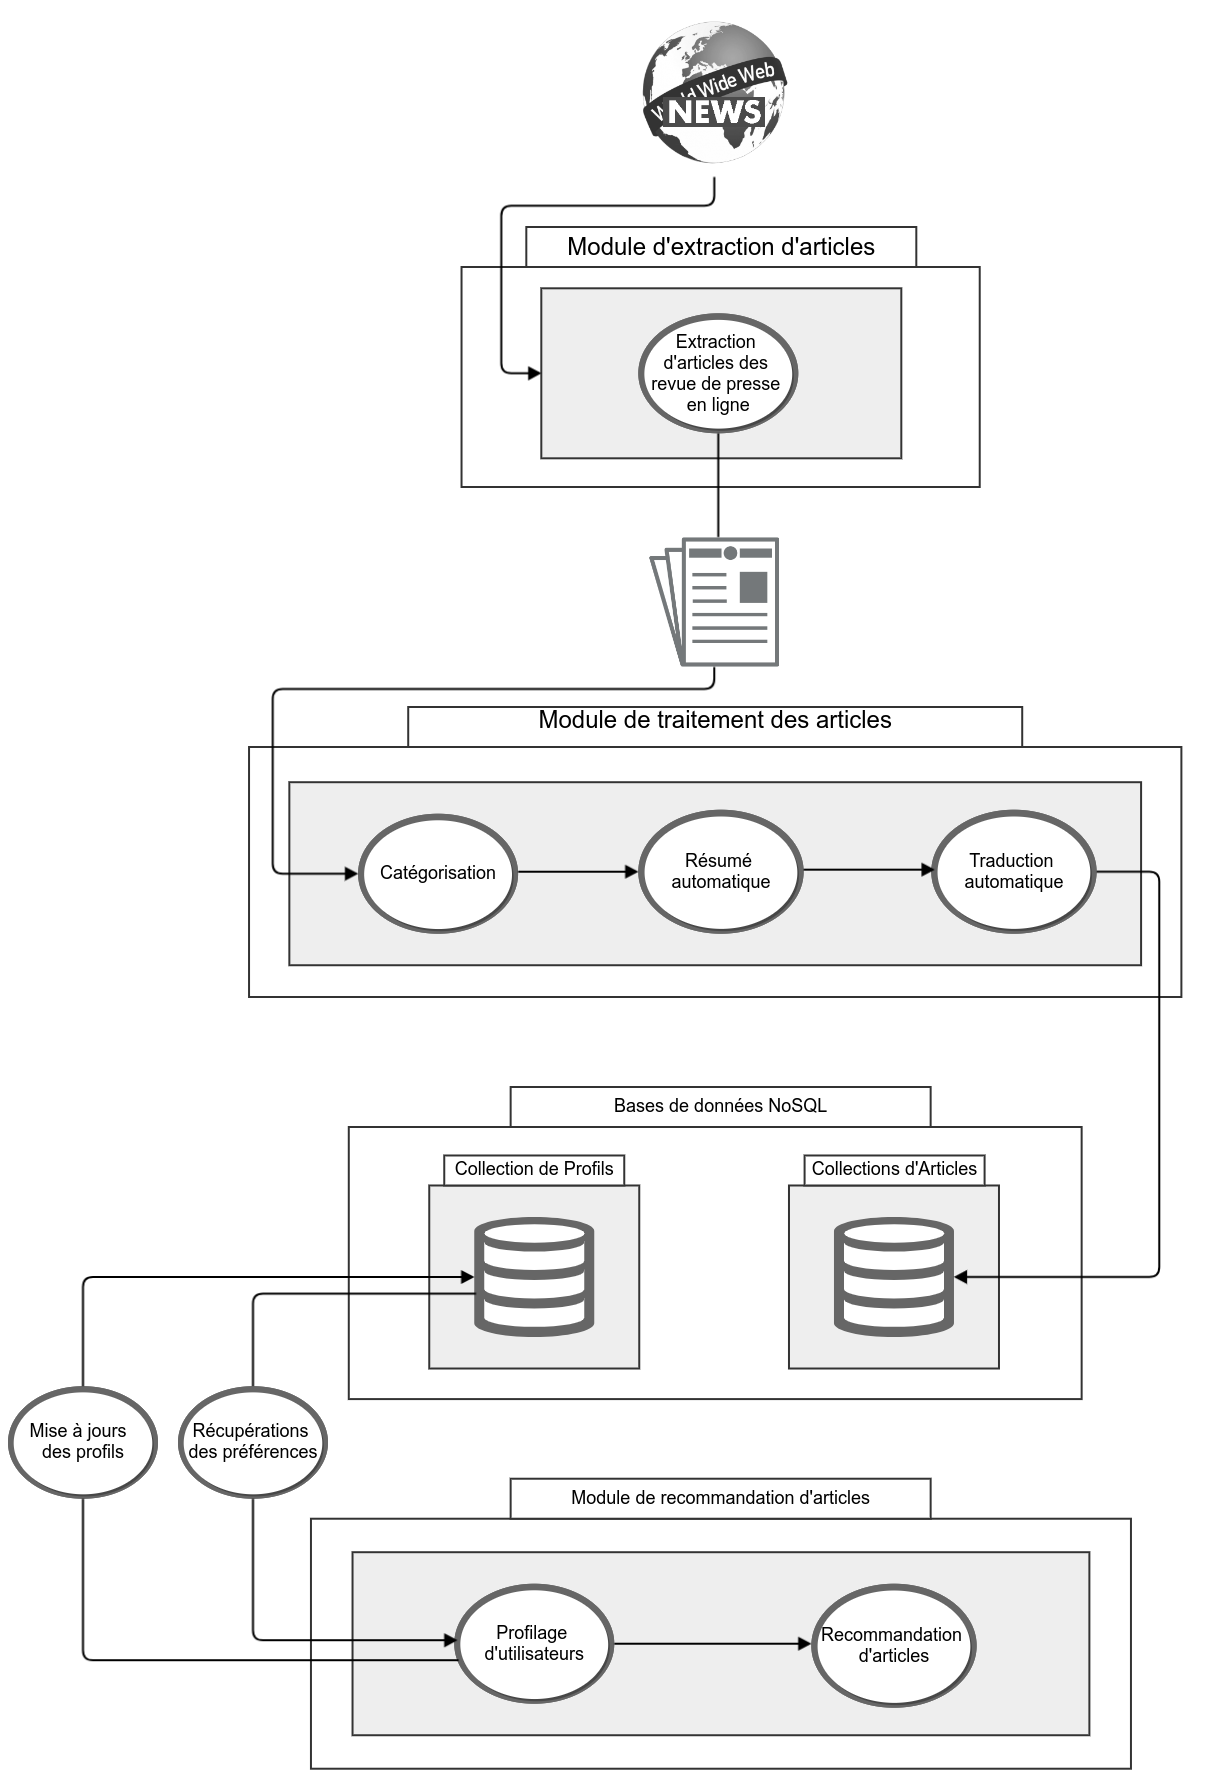
\includegraphics[height=520pt,width=380pt]{img/chapter3/global.png}
    \caption{Schéma global du fonctionnement de \textquotedbl Feedny\textquotedbl }
    \label{shemaglobal}
\end{figure}

\section{Schémas conceptuels de \textquotedbl Feedny\textquotedbl }
Nous allons présenter dans cette partie, la façon avec laquelle le logiciel fournit les différentes fonctionnalités. Celle-ci décrit d'une manière claire et précise, le fonctionnement du futur système en utilisant un langage de modélisation. Nous avons choisi la méthode UML (Unified Modeling Language), qui est une notation graphique conçue pour représenter, spécifier et construire les systèmes logiciels \cite{UML}.

\subsection{Diagramme de cas d'utilisation}
\textquotedbl Le diagramme de cas d'utilisation (initié par Ivar Jacobson en 1992 dans la méthode OOSE) est un type de diagramme UML qui permet de définir les besoins des acteurs dans un système quelconque en établissant les fonctionnalités attendues et en organisant les besoins. Il peut être aussi utilisés ensuite comme moyen d'organisation du développement du logiciel, notamment pour la structuration et le déroulement des tests du logiciel\textquotedbl\text{ }\cite{UML}.
\begin{figure}[H]
    \centering
    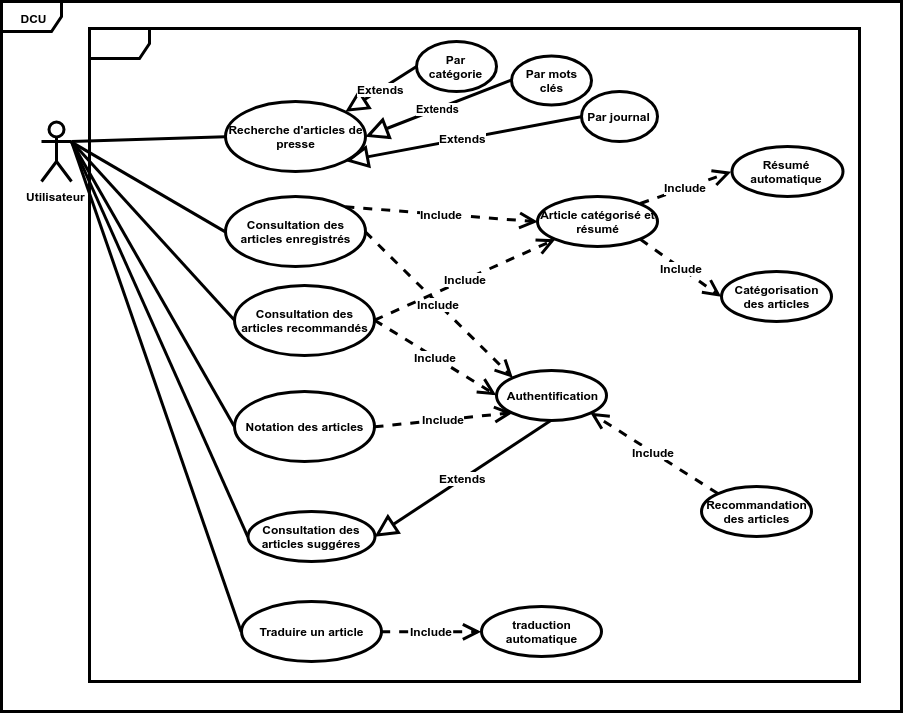
\includegraphics[height=400pt,width=350pt]{img/chapter3/diagcasdutilisation.png}
    \caption{Diagramme présentant les cas d'utilisations dans \textquotedbl Feedny\textquotedbl }
\end{figure}

\subsection{Diagramme de séquence}
Le diagramme de séquence est un diagramme UML qui fait partie des diagrammes comportementaux (dynamiques) dont L'objectif est de représenter les interactions entre les objets et les acteurs ou bien entre objets uniquement en indiquant la chronologie des échanges. Cette représentation peut se réaliser en considérant les différents scénarios associés \cite{UML}.
\begin{figure}[H]
    \centering
    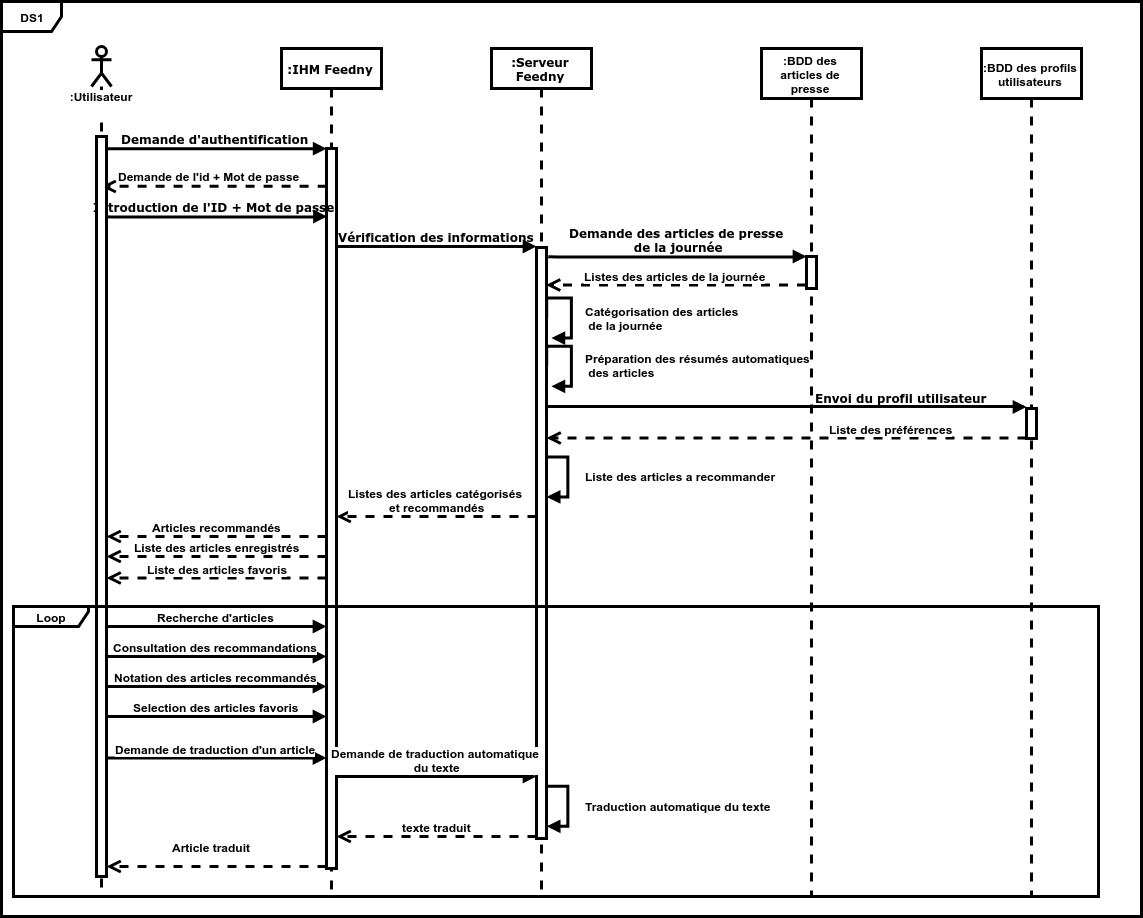
\includegraphics[height=500pt,width=425pt]{img/chapter3/diagseqperso.png}
    \caption{Diagramme de séquence de \textquotedbl Feedny\textquotedbl dans le cas personnalisée }
\end{figure}

\begin{figure}[H]
    \centering
    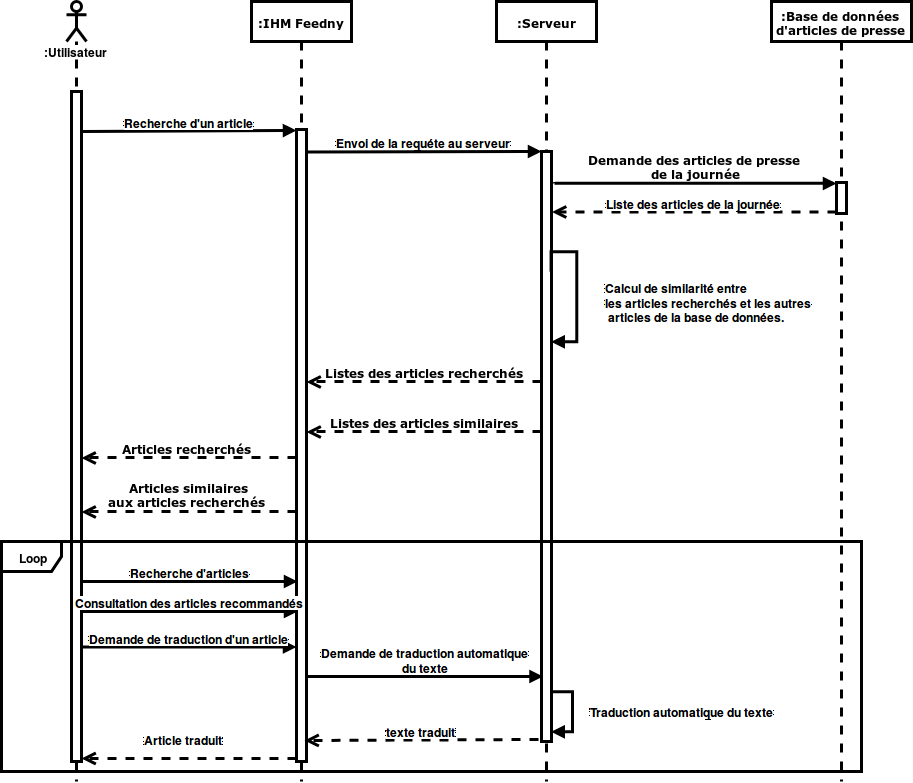
\includegraphics[height=500pt,width=425pt]{img/chapter3/diagseqnonperso.png}
    \caption{Diagramme de séquence de \textquotedbl Feedny\textquotedbl dans le cas non personnalisée }
\end{figure}

\section{Mesures d'évaluation du système}
L'évaluation de chaque module du système est l'une des étapes les plus importantes. Plusieurs métriques d'évaluations ont été utilisées, nous allons les présenter dans ce qui suit.

    \subsection{Métriques d'évaluation du module de recommandation}
    Pour évaluer le système de recommandation, il existe deux métriques principales, le \emph{RMSE} (Root mean squared error) et le \emph{MAE} (Mean absolute error). On va les présenter brièvement dans le point suivant. 

        \subsubsection{Métrique d'évaluation MAE}
        La moyenne erreur absolue (MAE) est une mesure largement utilisée dans les évaluations des modèles de recommandations. Elle est utilisée pour estimer la différence moyenne entre la note réelle et celle que le système de recommandation va prédire. 

        Plus la valeur du MAE est basse, plus la précision sera meilleure. En général, la valeur du MAE peut aller de 0 à l'infini, où l'infini est l'erreur maximale en fonction de l'échelle de notation de l'application mesurée \cite{rmse}. Le calcul de l'erreur absolue moyenne est fait comme suit :

        \[MAE = \frac{1}{n}\sum_{t=1}^{n}|d\textsubscript{i}|-|D\textsubscript{i}|\]

        Où d\textsubscript{i} est la note actuelle, D\textsubscript{i} est la note prédite et n est le nombre de notes.

        \subsubsection{Métrique d'évaluation RMSE}
        L'erreur quadratique moyenne (RMSE) a été utilisée comme mesure statistique standard pour mesurer la performance d'un modèle de recommandation. Elle  calcule la valeur moyenne de toutes les différences au carré entre les notes réelles et prédites. 

        En conséquence, de grandes erreurs peuvent affecter considérablement la note RMSE \cite{rmse}. La formule de calcul est la suivante :

        \[RMSE = \sqrt{\frac{1}{n}\sum_{t=1}^{n}(d\textsubscript{i} - D\textsubscript{i})^2}\] \\

        Où d\textsubscript{i} est la note actuelle, D\textsubscript{i} est la note prédite et n est le nombre de notes.

    \subsection{Métriques d'évaluation du module de catégorisation}
    Dans le module de catégorisation des articles, nous allons évaluer nos modèles en utilisant la précision, le rappel, la F-mesure et les tables de confusions \cite{mesurecateg}.
        \subsubsection{La matrice de Confusion}
        Pour analyser plus finement la qualité des classes produites par le modèle de catégorisation, on peut s’intéresser aux tables de confusion.

        Une matrice de confusion ou tableau de contingence sert à évaluer la qualité d'une classification. Elle est obtenue en comparant les données classées avec des données de référence qui doivent être différentes de celles ayant servi à réaliser la classification.
        
        \begin{itemize}
            \item{\textbf{TP }True Positive (vrais positifs) :} résultat où le modèle prédit correctement la classe positive.
            \item{\textbf{FP }False Positive (faux positifs) :} résultat où le modèle prédit incorrectement la classe positive.
            \item{\textbf{FN }False Negative (faux négatifs) :} résultat où le modèle prédit incorrectement la classe négative.
            \item{\textbf{TN }True Negative (vrais négatifs) :} résultat où le modèle prédit correctement la classe négative.
        \end{itemize}
        
        \subsubsection{Accuracy} 
        C'est une mesure qui évalue l'efficacité globale de l'algorithme par rapport au données de test.
        \[ Accuracy = \frac{tp+tn} {tp+fp+tn+fn} \]
        \subsubsection{Précision} 
        Elle évalue le pouvoir prédictif du modèle en mesurant la capacité du modèle à prédire que des classes correctes.
        \[ Precision = \frac{tp} {tp+fp} \]
        \subsubsection{Rappel} 
        La capacité d’un modèle à prédire toutes les classes correctes de l'ensemble de test.
        \[ Rappel = \frac{tp} {tp+fn} \]
        \subsubsection{F-mesure}
        Une mesure composite qui profite aux algorithmes avec une sensibilité plus élevée et des algorithmes de défis avec spécificité plus élevée. \label{fmesure}
        \[ F-mesure = \frac{2 * (Precision * Rappel)} {(Precision + Rappel)}\]
        
        \subsubsection{Courbe ROC} 
        C'est une course qui montre la relation entre la sensibilité et la spécificité de l'algorithme.
        
        \subsubsection{Perplexité}
        Dans le traitement du automatique du langage naturel, la perplexité est un moyen d'évaluer les modèles de langage \cite{perplexite}. Un modèle de langage est une distribution de probabilité sur des phrases ou des textes entiers. Elle est calculée comme suit:
        \[
        \text{perplexite}(D\textsubscript{test}) =
        \exp
        \left \{-\frac{\sum_{d=1}^{M}{\log{p(w_d)}}}{\sum_{d=1}^{M}{N_d}}\right\}
        \]

        Où D est un document, w est un terme du document, p(w) est la probabilité d'apparition du terme w dans D et N est le nombre de mots dans le document.

        La valeur de celle-ci est algébriquement équivalente à l'inverse de la moyenne géométrique par vraisemblance. Un score de perplexité inférieur indique une meilleure performance de généralisation.

        \subsubsection{Cohérence de sujet}
        La cohérence de sujet (Topic coherence) mesure le , dans les mots utilisés pour décrire une catégorie, un mot commun est en moyenne un bon prédicteur pour un mot moins commun.

        Nous allons calculer la cohérence en utilisant \textquotedbl intrinsic UMass measure\textquotedbl qui est proposé par \cite{perplexite}. La formule est présentée là-dessous :
        \[
        \text{score}_{\text{UMass}}(w_i, w_j) =
        \log
        \frac{D(w_i, w_j) + 1}{D(w_i)}
        \]
        Où w\textsubscript{i} est un mot commun et w\textsubscript{j} est moins commun, les deux mots font parti des mots qui décrivent une catégorie, D est un document.

    \subsection{Métriques d'évaluation du module de résumé automatique}
    Dans le module de résumé automatique, la mesure principale est \emph{Rouge}. Ci-dessous, nous allons la présenter.

        \subsubsection{Métrique d'évaluation ROUGE\label{metrique-eval}}
        ROUGE est l'acronyme de \textquotedbl Recall-Oriented Understudy for Gisting Evaluation\textquotedbl. Il s'agit essentiellement d'un ensemble de métriques permettant d'évaluer le résumé automatique de textes ainsi que la traduction automatique. Il fonctionne en comparant un résumé produit automatiquement ou une traduction à un ensemble de résumés de référence (généralement produits par des humains) \cite{rouge0}.

        \subsubsection{Types des métriques de ROUGE\label{type-rouge}}
        \begin{itemize}
            \item{ROUGE-1, 2, 3 et 4 : font référence au chevauchement des uni-grammes, bi-grammes, tri-grammes et quadri-grammes, respectivement, entre le système et les résumés de référence \cite{rouge1}.}\\
            \item{ROUGE-L, W : basés sur la plus longue sous-séquence commune (LCS) \cite{rouge2}.}\\
            \item{ROUGE-S : basé sur les cooccurrences des paires de mots dans l'ordre des phrases \cite{rouge2}.}\\
            \item{ROUGE-SU : en plus des paires de mots, il utilise aussi la cooccurrence du mot unique toujours dans l'ordre des phrases.}
        \end{itemize}

        Les métriques citées dans la \autoref{type-rouge}, utilisent comme mesures le rappel, la précision et la f-mesure, déjà présentées. Dans ce qui suit, nous allons donner des explications de l'utilisation de chaque métrique :  
        \begin{itemize}
            \item {Le rappel dans le cas de ROUGE, donne une information sur le nombre de mots du résumé de référence ont été capturés par le résumé de notre généré par le système.\\ 
                Exemple: si le rappel est égal a 40\%, cela signifie que 40\% des n-grammes du résumé de référence sont également présents dans le résumé généré par le système.}\\
            \item {La précision quant à elle, mesure la partie du résumé du système qui est pertinente ou nécessaire.\\ 
                Exemple : si la précision est égale a 40\%, cela signifie que 40\% des n-grammes du résumé généré par le système sont également présents dans le résumé de référence.}
            \item {La F-mesure est calculée à partir de la précision et du rappel \ref{fmesure}.}
        \end{itemize}

\section{Conclusion}
Lors de ce chapitre, nous avons proposé la conception du système \textquotedbl Feedny\textquotedbl. Nous avons commencer par décrire la conception des modules de recommandation, de catégorisation d'articles, de résumé et de la traduction automatique. Nous avons ensuite décrit la structure de notre base de données, puis présenter l'architecture globale du système. Par la suite, nous avons présenter les schémas conceptuels de \textquotedbl Feedny\textquotedbl. Et nous avons, enfin, expliciter les mesures d'évaluation des différents modules. Dans le prochain chapitre, nous allons présenter la réalisation et les résultats de notre travail.